\documentclass[12pt, a4paper, oneside]{article}

\usepackage[brazil]{babel}
\usepackage[utf8]{inputenc}
\usepackage[T1]{fontenc}
\usepackage{graphicx}
\usepackage{url}
\usepackage{array}
\usepackage{times}
\usepackage{setspace}
\usepackage{color}
\usepackage{booktabs}
\usepackage{rotating}


\usepackage[square,numbers]{natbib}

\renewcommand*\thesection{\arabic{section}}

%\hyphenation{}

\begin{document}


\title{\textbf{Filtragem Colaborativa Baseada em Itens}\\
	\normalsize{Relatório do Trabalho Prático 2 -- Sistemas de Recomendação -- 2014.2}
}

\author{
    \textbf{Aécio Solano Rodrigues Santos}\\ 
    \small{\texttt{aeciosantos@dcc.ufmg.br}}\\
    \and
    \textbf{\small{Universidade Federal de Minas Gerais}}\\
    \small{Departamento de Ciência da Computação}\\
    \small{Belo Horizonte, Brasil}
}

\date{}

\maketitle

%\onehalfspacing

%------------------------------------------------------------------------------

\section{Introdução}
\label{sec:introducao}

Filtragem Colaborativa é um dos métodos clássicos utilizados por sistemas de recomendação para gerar recomendações de item personalizadas para cada usuário.
A abordagem de filtragem colaborativa baseada em item é uma técnica que tem ficado bastante popular devido à qualidade das recomendações e à escalabilidade do método para grandes bases de dados devido à possibilidade de computação de um modelo \textit{offline}.

Neste trabalho é apresentado a implementação e avaliaç\~ao de um algoritmo clássico de filtragem colaborativa baseada em item (\textit{Item-to-Item Colaborative Filtering}). O algoritmo foi implementado usando linguagem Java 8 e avaliado utilizando a base de dados Movie Lens 100k.

Os experimentos apresentados mostram a influência da quantidade de itens similares na acurácia do algoritmo nas tarefas de predição de ratings e recomendação de uma lista de itens de recomendação. É feito ainda uma comparação entre o algoritmo de filtragem colaborativa baseada em item com um algoritmo não personalizado simples, e com um algoritmo de filtragem colaborativa baseado em usuário implementado no trabalho prático anterior.

%Os resultados mostram uma melhora da acurácia na predição dos ratings da abordagem personalizada de acordo com a métrica RMSE (\textit{Root Mean Square Error}).

O restante do trabalho está organizado da seguinte forma. A descrição do algoritmo implementado é apresentado na seç\~ao \ref{sec:algoritmo}. A base de dados utilizada é descrita brevemente na seç\~ao \ref{sec:dataset}. Os experimentos realizados e resultados serão apresentados na seção \ref{sec:experimentos}. Por fim, na seç\~ao \ref{sec:conclusao} constar\'a as conclus\~oes e consideraç\~oes finais.


%------------------------------------------------------------------------------

\section{Algoritmo de Filtragem Colaborativa}
\label{sec:algoritmo}

Esta seção apresenta uma breve descrição do algoritmo de filtragem colaborativa
baseada em item utilizado para fazer a predição de ratings.
A premissa básica de métodos de recomendação baseados em filtragem colaborativa é 
que as pessoas tem preferências similares, ou seja, a opinião de outros usuários pode ser
agregada de forma a prover predições das preferencias do usuário para que ser quer
fazer uma recomendação \cite{ekstrand2011collaborative}.



\subsection{Item-to-Item Colaborative Filtering (IICF)}
\label{sec:item-to-item}

% intro
Diferentemente do filtragem colaborativa baseada em usuário, que utiliza a matriz de 
iteração entre itens e usuários para computar a similaridade de usuários e em seguida
recomendar itens que usuários semelhantes também gostaram, a filtragem colaborativa 
baseada em item analiza a matriz de ratings partindo da perspectiva de itens. Primeiro
são computadas o similaridades entre os diversos itens levando em conta as preferências
das pessoas que avaliaram os itens, e a partir daí a predição é computada baseada nos
ratings em itens similares aos itens que um usuário já manifestou sua preferência no passado.

% similaridade de items
O primeiro passo do algoritmo IICF é obter uma matriz de similaridade entre cada par de itens
da base de dados. Existem diversas métricas de similaridade que podem ser utilizadas para
computar a semelhança entre dois itens $a$ e $b$. Uma forma comumente utilizada para calcular
a similaridade é representar cada item como um vetor e computar o valor do cosseno entre os 
dois vetores. Esse vetor é composto pelos ratings dos usuários em cada item, ou seja,
o vetor $A$, que representa o item $a$, é um vetor $|U|$-dimensional em que $A[u]$ é o rating do usuário $u$ no item $a$. Formalmente,
$$sim(a,b) = \frac{A \cdot B}{|A| |B|} = \frac{ \sum\limits_{u \in U} r_{a,u} r_{b,u} }{ \sqrt{ \sum\limits_{u \in U} r_{a,u}^2 } \sqrt{ \sum\limits_{u \in U} r_{b,u}^2 } } $$
em que $A \cdot B$ é o produto escalar entre os vetores $A$ e $B$;  $|A|$ e $|B|$ são as normas dos vetores; $r_{a,u}$ é o rating do usuário $u$ no item $a$; e $U$ é o conjunto de usuários que avaliaram os itens $a$ e $b$.

Uma alternativa à similaridade do cosseno, é ajustar o valor dos ratings subitraindo os valores dos ratings $r$ na fórmula anterior, pela médias dos ratings do usuário $u$.

% similaridade conseno ajustada
% ?

% blablabla
Apesar de ser uma operação relativamente cara, a computação da similaridade entre cada par de itens pode ser feita em um processo offline para melhorar o tempo da computação da recomendação on-line.

% computação da predição
% ?
Finalmente, para computar a predição dos ratings, o IICF usa uma média ponderada dos ratings dos $k$ itens mais similares aos itens avaliados pelo usuário, como segue:

$$ pred(u, i) = \frac{ \sum_{p^\prime \in ratedItems(U)} sim(i,p) r_{p, u}) }{ \sum_{p^\prime \in ratedItems(U)} |sim(i,p)| } $$


%\pagebreak

%------------------------------------------------------------------------------
\section{Dataset}
\label{sec:dataset}
Para avaliar o algoritmo foi utilizada a base dados MovieLens 100k. Esta base contém 100,000 ratings
com escala de 1 a 5 dados por 943 usuários para 1682 filmes. Cada usuário avaliou pelo menos 20 filmes.
Além disso, a base contém informações demográficas simples sobre os usuários, porém essas informações 
não foram utilizadas neste trabalho. O Dataset está publicamente disponível em \texttt{http://grouplens.org/datasets/movielens/}.
%------------------------------------------------------------------------------
\section{Experimentos}
\label{sec:experimentos}

O primeiro experimento realizado teve o objetivo de identificar como o tamanho da vizinhança de itens similares
influencia a eficácia do algoritmo. Nesse experimento utilizou-se a o arquivo \texttt{ua.base} para o
treinamento do algoritmo, e o arquivo \texttt{ua.test} para computar a acurácia.
A acurácia é foi medida utilizando duas métricas:
\begin{itemize}
\item \textbf{RMSE} (Root Mean Squared Error), dada por:
$$ RMSE = \sqrt{ \frac{1}{n}\sum_{i=1}^n(\hat{Y_i} - Y_i)^2} $$
onde $\hat{Y_i}$ é o rating calculado pelo algoritmo e $Y_i$ é o rating real que o usuário deu para o item $i$.
\item \textbf{MAP} (Mean Average Precision), dada por:

$$ MAP = \frac{ \sum\limits_{q \in Q} AP(q) }{ |Q| }$$
em que $Q$ é conjunto de listas de recomendações a serem avaliadas; $AP(q)$ é a Precisão Média (\textit{Average Precision}) da lista de recomendação $q$; $|Q|$ é a quantidade listas de recomendações no conjunto $Q$; e a precisão média $AP$ é dada por:
$$ AP = \frac{ \sum\limits_{k=1}^n P(k) \times rel(k) }{ \mbox{número de itens relevantes}} $$
onde $P(k)$ é a precisão no ponto de corte $k$ na lista de recomendações e $rel(k)$ é uma função indicadora igual a $1$ quando o item da posição, e igual a $0$ caso contrário.
\end{itemize}

A Figura \ref{fig:rmse} mostra o resultado da variação do valor de número de itens similares. A medida que o número de itens, $k$, aumenta, a acurácia melhora rapidamente e depois se mantém estável. O algoritmo que obteve melhores resultados foi o de filtragem colaborativa baseada em usuário (\textit{User-User}), enquanto o algoritmo de filtragem colaborativa baseada em item utilizado a similaridade de cosseno ajustada não obteve bons resultados. Esses resultados indicam que o algoritmo baseado em usuário obtém melhores resultados na tarefa de predição de ratings.

%\pagebreak

\begin{figure}[!ht]
\centering
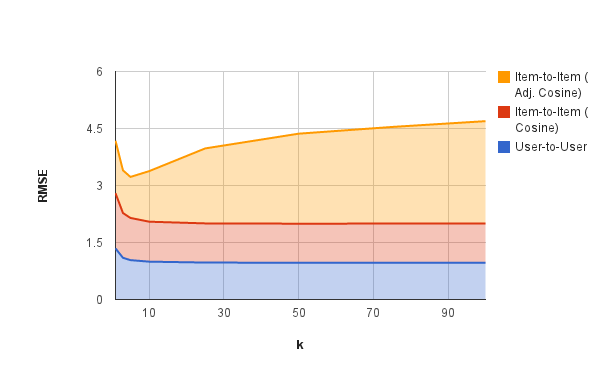
\includegraphics[scale=.45]{img/rmse.png} 
\caption{Influência de valores de $k$ na acurácia de predições em termos de RMSE}
\label{fig:rmse}
\end{figure}

\begin{figure}[!ht]
\centering
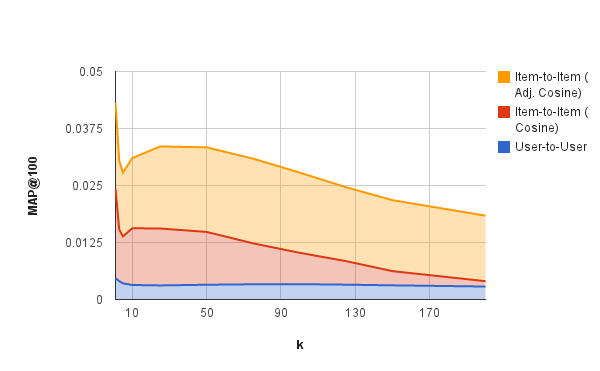
\includegraphics[scale=.45]{img/map.png} 
\caption{Influência de valores de $k$ na acurácia de predições em termos de MAP}
\label{fig:map}
\end{figure}

A Figura \ref{fig:map} mostra os resultados dos algoritmos, em termos de MAP, a medida que o valor de $k$ varia. Neste experimento, os algoritmos baseados em item obtiveram uma precisão melhor do que o algoritmo baseado em usuário. Esses resultados indicam que apesar de o algoritmo baseado em usuário ser melhor na tarefa de predição de ratings, os algoritmos baseados em itens podem ser melhores quando a tarefa é recomendação de uma lista de itens.


A Figura \ref{fig:baselines-rmse} mostra o resultado dos melhores valores encontrados para cada algoritmo junto com um
algoritmo simples não personalizado que considera a média de ratings do item predição. Com, exceção do algoritmo baseado em item utilizando similaridade de cosseno ajustada (IICF k=5 Adj. Cos.), todos os outros conseguiram superar o baseline não personalizado.

\begin{figure}[!ht]
\centering
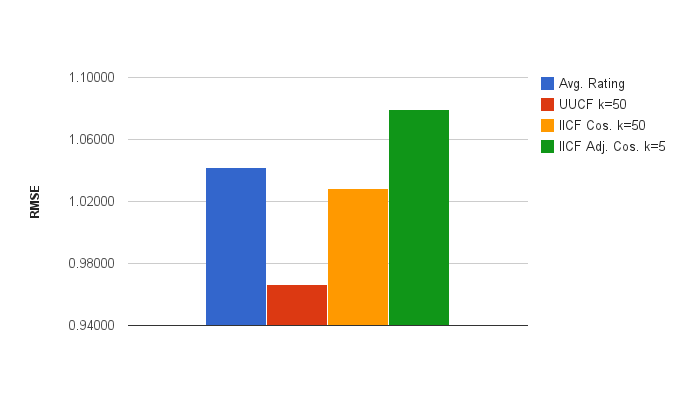
\includegraphics[scale=.45]{img/baseline-rmse.png} 
\caption{Melhores resultados em termos de RMSE}
\label{fig:baselines-rmse}
\end{figure}


%------------------------------------------------------------------------------
\section{Conclusão}
\label{sec:conclusao}
Nesse trabalho, descrevemos o algoritmo de filtragem colaborativa baseado em item (Item-Item Colaborative Filtering) e apresentamos um estudo sobre a influência da quantidade de itens similares na acurácia do algoritmo. Foi feito ainda uma comparação da acurácia do algoritmo baseado item com um algoritmo de filtragem colaborativa baseado em usuário e outro não personalizado. Os resultados mostram que cada algoritmo pode ser melhor dependendo da tarefa de recomendação desejada: predição de ratings ou recomendação de uma lista de itens.
%------------------------------------------------------------------------------

\bibliography{tp}
\bibliographystyle{plain}

\end{document}
